\documentclass[12pt,a4paper]{article}

%====================================================
%                  PACKAGES
%====================================================
\usepackage{graphicx}
\usepackage{subcaption}
\usepackage{fancyhdr}
\usepackage[margin=1in]{geometry}
\usepackage{listings}
\usepackage[hidelinks]{hyperref}
\usepackage{amsmath,amssymb,mathtools}
\usepackage{float}
\usepackage{lmodern}
\usepackage{xcolor}
\usepackage{fvextra}
\usepackage{longtable}
\usepackage{enumitem}
\usepackage{booktabs}
\usepackage{array}
\usepackage{multirow}
\usepackage{colortbl}
\usepackage{titlesec}
\usepackage{tikz}
\usepackage{eso-pic} 
\usepackage[most]{tcolorbox}
\usepackage{xepersian}
\usetikzlibrary{calc} 

%====================================================
%                  COLORS
%====================================================
% رنگ‌های پایه
\definecolor{mainblue}{RGB}{15,76,129}
\definecolor{lightblue}{RGB}{226,238,250}
\definecolor{deepblue}{RGB}{9,24,51} 
\definecolor{darkpurple}{RGB}{60,20,80} 

% رنگ‌های ملایم و پاستلی برای باکس‌ها (کمرنگ و خفن)
\definecolor{softgreen}{RGB}{240,250,245}
\definecolor{mygreen}{RGB}{46,139,87}

\definecolor{softorange}{RGB}{255,248,235}
\definecolor{golden}{RGB}{218,165,32} 

\definecolor{softpink}{RGB}{255,240,245}
\definecolor{softred}{RGB}{205,92,92}

\definecolor{softgray}{RGB}{248,248,248}
\definecolor{glassbg}{RGB}{255,255,255} 

%====================================================
%                  HYPERREF
%====================================================
\hypersetup{
	colorlinks=true,
	linkcolor=mainblue, 
	filecolor=magenta,
	urlcolor=mainblue, 
	citecolor=mygreen 
}

%====================================================
%                  FONTS
%====================================================
\settextfont[Path={./font/}, Scale=1.3]{IRLotus}
\setlatintextfont[Scale=1]{Times New Roman}

%====================================================
%                  PAGE STYLE
%====================================================
\setlength\headheight{28pt}
\pagestyle{fancy}
\fancyhf{}
\lhead{\textcolor{mainblue}{\textbf{پروژه هوش مصنوعی}}}
\chead{
\includegraphics[width=1cm,height=1cm,keepaspectratio]{img/Logo.png}}
\rhead{\textcolor{mainblue}{\textbf{\thepage}}}
\rfoot{\textcolor{gray}{حامد بهروزی مقدم - علیرضا دیوسالار}}
\renewcommand{\headrulewidth}{1.5pt} 
\renewcommand{\headrule}{\hbox to\headwidth{\color{mainblue}\leaders\hrule height \headrulewidth\hfill}}
\renewcommand{\footrulewidth}{1pt}
\renewcommand{\footrule}{\hbox to\headwidth{\color{gray}\leaders\hrule height \footrulewidth\hfill}}

%====================================================
%                  SECTION STYLE
%====================================================
\titleformat{\section}
{\Large\bfseries\color{mainblue}}
{\begin{tikzpicture}[baseline={(0,-0.1)}]
		\node[fill=mainblue,text=white,rounded corners=2pt,inner sep=4pt] {\thesection};
\end{tikzpicture}}
{0.5em}
{}[\vspace{0.2ex}\titlerule] 

\titlespacing{\section}{0pt}{20pt}{10pt} 

%====================================================
%                  LINE SPACING & LISTINGS
%====================================================
\renewcommand{\baselinestretch}{1.5}

\definecolor{codegreen}{rgb}{0,0.55,0}
\definecolor{codegray}{rgb}{0.45,0.45,0.45}
\definecolor{codepurple}{rgb}{0.58,0,0.82}
\definecolor{backcolour}{rgb}{0.97,0.97,0.94}

\lstdefinestyle{mystyle}{
	backgroundcolor=\color{backcolour},
	commentstyle=\color{codegreen},
	keywordstyle=\color{magenta},
	numberstyle=\tiny\color{codegray},
	stringstyle=\color{codepurple},
	basicstyle=\ttfamily\footnotesize,
	breakatwhitespace=false,
	breaklines=true,
	captionpos=b,
	keepspaces=true,
	numbers=left,
	numbersep=6pt,
	showspaces=false,
	showstringspaces=false,
	showtabs=false,
	tabsize=4,
	frame=shadowbox, 
	rulesepcolor=\color{mainblue}
}
\lstset{style=mystyle}

%====================================================
%                  TCOLORBOX
%====================================================
\tcbset{
	enhanced,
	breakable,
	arc=3mm, 
	boxrule=1pt, 
	fonttitle=\bfseries\large, 
	drop fuzzy shadow 
}

%====================================================
%                  AUTOREF
%====================================================
\AtBeginDocument{
	\def\chapterautorefname{فصل}%
	\def\sectionautorefname{بخش}%
	\def\subsectionautorefname{زیربخش}%
	\def\equationautorefname{رابطه}%
	\def\figureautorefname{شکل}%
	\def\tableautorefname{جدول}%
}

%====================================================
%                  DOCUMENT
%====================================================
\begin{document}
	
	%====================================================
	%                  TITLE PAGE
	%====================================================
	
	\begin{titlepage}
		\AddToShipoutPictureBG*{
			\begin{tikzpicture}[remember picture,overlay]
				\fill[deepblue] (current page.south west) rectangle (current page.north east);
				\shade[top color=white, bottom color=white, opacity=0.08] 
				(current page.north west) rectangle ($(current page.north east)+(0,-6cm)$);
				\fill[white, opacity=0.03] (current page.north west) circle (8cm);
				\fill[white, opacity=0.02] (current page.south east) circle (12cm);
				\fill[white, opacity=0.04] (current page.north east) +(-4cm,-4cm) circle (6cm);
				\fill[white, opacity=0.03] (current page.south west) +(4cm,4cm) rectangle +(8cm,8cm);
				\fill[white, opacity=0.02] (current page.center) circle (5cm);
				
				\draw[white, ultra thick, rounded corners=15pt, opacity=0.7] 
				($(current page.north west)+(1.5cm,-1.5cm)$) rectangle ($(current page.south east)+(-1.5cm,1.5cm)$);
				\draw[white, thick, dashed, opacity=0.2] 
				($(current page.north west)+(1.7cm,-1.7cm)$) rectangle ($(current page.south east)+(-1.7cm,1.7cm)$);
			\end{tikzpicture}
		}
		
		\begin{center}
			\vspace*{1.5cm} 
			
			{\fontsize{30}{35}\selectfont \textbf{\textcolor{white}{پیش‌بینی هوشمند هزینه‌های حق بیمه پزشکی}}} 
			
			\vspace{0.8cm} 
			
			{\LARGE \textbf{\textcolor{white}{درس هوش مصنوعی}}} 
			
			\vspace{1cm} 
			
			\begin{tcolorbox}[
				colback=white,       
				colframe=white,      
				boxrule=0pt,         
				arc=3mm,             
				left=2mm, right=2mm, top=2mm, bottom=2mm, 
				width=0.2\textwidth, 
				halign=center        
				]
				
\includegraphics[width=\linewidth]{img/Logo.png}
			\end{tcolorbox}
			
			\vspace{1.2cm} 
			
			\begin{tcolorbox}[
				width=0.85\textwidth,
				colback=white, 
				opacityback=0.1, 
				colframe=white, 
				coltitle=blue, 
				title={\Large \textbf{فاز اول پروژه پایانی}}, 
				halign title=center,
				halign=center,
				arc=5mm, 
				boxrule=1.5pt, 
				shadow={2mm}{-2mm}{0mm}{black!40} 
				]
				\large
				\textcolor{black}{طراحی و پیاده‌سازی جامع رگرسیون چندجمله‌ای، شبکه‌های عصبی عمیق پیشخور \lr{(MLP)} و پیاده‌سازی گام‌به‌گام سیستم استنتاج فازی-عصبی تطبیقی \lr{(ANFIS)} بر اساس مقاله کلاسیک \lr{Jang (1993)}.}
			\end{tcolorbox}
			
			\vspace{1cm} 
			
			\begin{tcolorbox}[
				width=0.75\textwidth,
				colback=white, 
				colframe=white, 
				arc=3mm,
				boxrule=2pt,
				halign=center,
				shadow={1mm}{-1mm}{0mm}{black!20} 
				]
				\renewcommand{\arraystretch}{1.5} 
				\large
				\begin{tabular}{>{\bfseries\color{mainblue}}l l} 
					نام دانشجو: & حامد بهروزی مقدم (\lr{40215633}) \\
					& علیرضا دیوسالار (\lr{40217493}) \\
					استاد درس: & جناب آقای دکتر علیاری \\
				\end{tabular}
			\end{tcolorbox}
			
		\end{center}
	\end{titlepage}
%====================================================
%                  INTRODUCTION
%====================================================

\section{مقدمه و تشریح کلی پروژه}

\begin{tcolorbox}[
	colback=softgreen,
	colframe=mygreen,
	title=هدف مهندسی پروژه,
	halign title=center,
	arc=3mm, boxrule=1pt
	]
	تبیین یک مدل ریاضی و هوشمند با تفسیرپذیری بالا و خطای اندک جهت پیش‌بینی نرخ عددی متغیر پیوسته حق بیمه سالیانه افراد بر اساس الگوهای فیچرهای دموگرافیک.
\end{tcolorbox}

مسئله تخمین حق بیمه پزشکی به دلیل ماهیت غیرخطی و رفتارهای سینگولار داده‌ها (به طور ویژه جهش ناگهانی هزینه‌ها برای افراد سیگاری با شاخص توده بدنی بالا) یکی از چالش‌های کلاسیک در حوزه یادگیری ماشین به شمار می‌رود. در حوزه‌های حساس مانند پزشکی و بیمه، تنها داشتن یک پیش‌بینی دقیق کافی نیست؛ بلکه **«تفسیرپذیری» (Interpretability)** مدل و توانایی توضیح دلایل پشت هر تصمیم به شدت حائز اهمیت است.

در این پروژه، ما با پیاده‌سازی سه رویکرد کاملاً متمایز شامل مدل‌های آماری خطی تعاملی، شبکه‌های عصبی متراکم \lr{(MLP)} به عنوان یک جعبه سیاه پیچیده، و در نهایت سیستم‌های تلفیقی عصبی-فازی \lr{(ANFIS)} به عنوان یک جعبه شیشه‌ای، موازنه میان معیارهای محاسباتی پایداری، دقت پیش‌بینی و قدرت تفسیرپذیری مدل‌ها را به صورت آزمایشگاهی تحلیل می‌نماییم.

%====================================================
%                  DATA PREPROCESSING
%====================================================

\section{پیش‌پردازش و تحلیل اکتشافی داده‌ها \lr{(EDA)}}

مجموعه داده‌های بیمه شامل ۱۳۳۸ رکورد است. برای آماده‌سازی این دیتاست، فرآیندهای مهندسی ویژگی زیر به صورت گام‌به‌گام در یک \lr{Pipeline} ایمن اعمال شده است:
\begin{itemize}
	\item \textbf{کدگذاری متغیرهای دودویی:} متغیرهای رشته‌ای نظیر جنسیت (\lr{sex}) و وضعیت دخانیات (\lr{smoker}) توسط \lr{LabelEncoder} به کدهای باینری صفر و یک نگاشت شدند.
	\item \textbf{تبدیل متغیرهای چندکلاسه:} ویژگی منطقه‌ای (\lr{region}) با متد \lr{One-Hot Encoding} بسط یافت و برای ممانعت از هم‌خطی چندگانه (\lr{Multicollinearity})، پارامتر \lr{drop\_first=True} اعمال گردید.
	\item \textbf{جلوگیری از نشت داده‌ها (\lr{Data Leakage}):} تقسیم‌بندی مجموعه به دو بخش آموزش و تست با نسبت ۸۰ به ۲۰ مستقیماً پیش از فاز مقیاس‌دهی انجام پذیرفت. سپس \lr{StandardScaler} منحصراً بر روی داده‌های آموزش \lr{fit} گردید تا هیچ اطلاعاتی از مجموعه تست وارد فاز آموزش نگردد.
\end{itemize}

\subsection{بصری‌سازی ساختار داده‌ها و توزیع ویژگی‌ها}
پیش از ورود به فاز مدل‌سازی، نمودارهای تحلیل اکتشافی برای بررسی ساختار توزیع متغیر هدف و تعاملات ویژگی‌های کلیدی ترسیم شدند.

\begin{figure}[H]
	\centering
	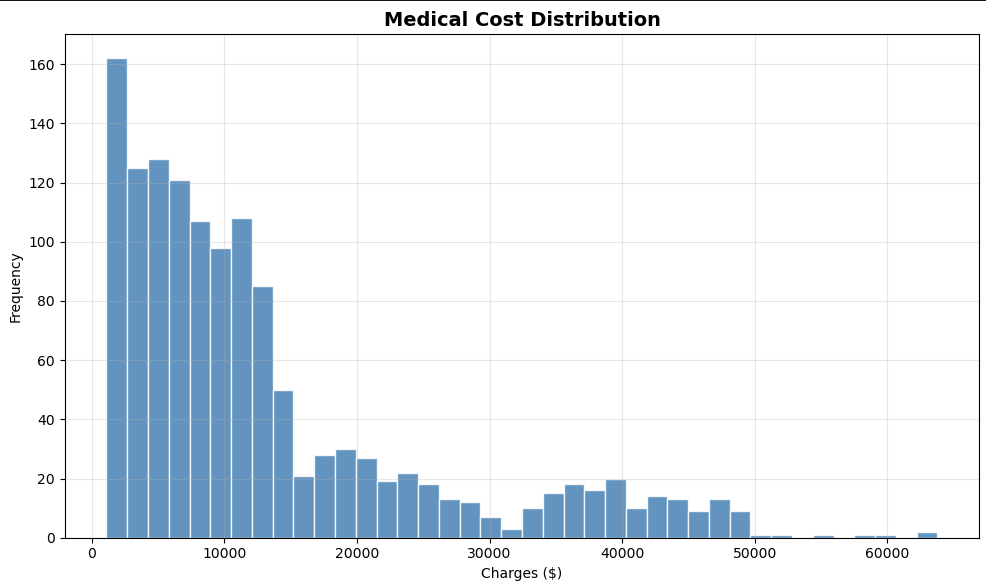
\includegraphics[width=0.75\textwidth]{fig1.png}
	\caption{نمودار \lr{fig1}: توزیع چگالی متغیر هدف (حق بیمه). انحراف شدید به سمت راست، گواه بر فراوانی هزینه‌های پایه و رخدادهای نادر با هزینه‌های سنگین است.}
\end{figure}

\begin{figure}[H]
	\centering
	\begin{subfigure}{0.48\textwidth}
		\centering
		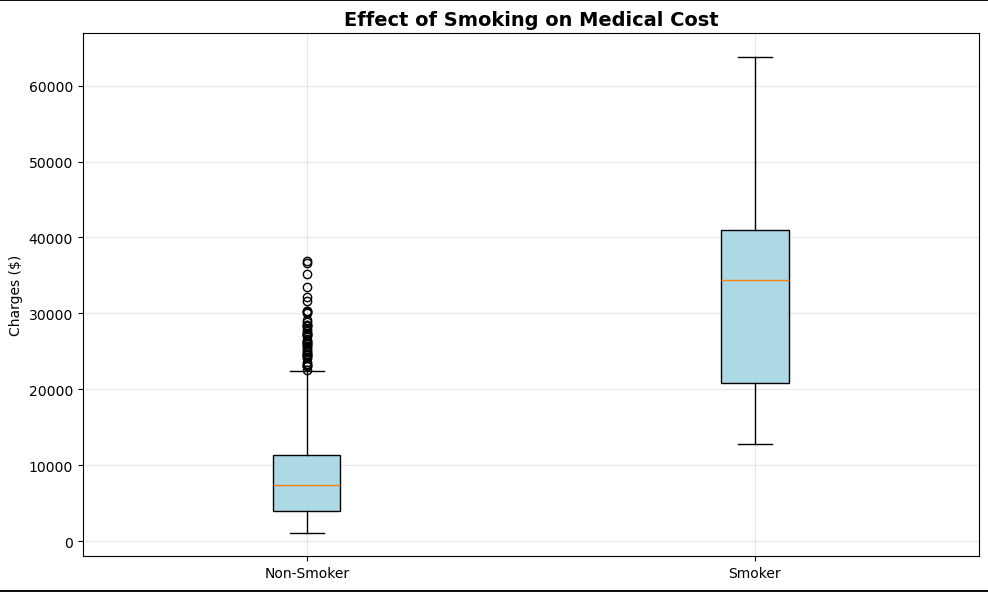
\includegraphics[width=\linewidth]{fig2.png}
		\caption{نمودار \lr{fig2}: تأثیر سهمگین مصرف سیگار بر حق بیمه.}
	\end{subfigure}\hfill
	\begin{subfigure}{0.48\textwidth}
		\centering
		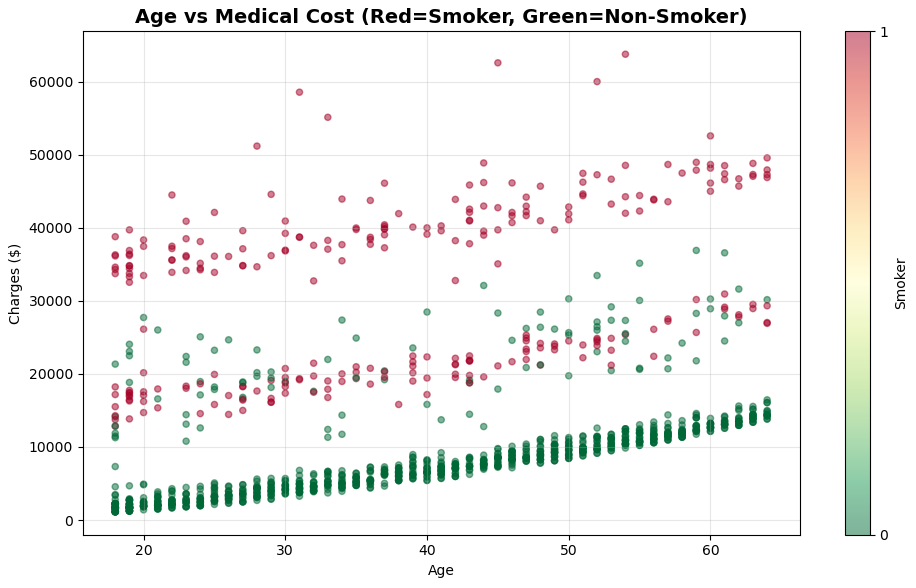
\includegraphics[width=\linewidth]{fig3.png}
		\caption{نمودار \lr{fig3}: پراکندگی سن و هزینه به تفکیک سیگار.}
	\end{subfigure}
	\caption{تحلیل اکتشافی داده‌ها: همان‌طور که مشهود است، متغیر مصرف سیگار باعث ایجاد یک شیفت (\lr{Shift}) خطی بسیار قدرتمند در هزینه‌های پایه افراد شده است.}
\end{figure}

%====================================================
%                  PHASE 1: REGRESSION
%====================================================

\section{فاز اول: رگرسیون خطی و تعاملی (چندجمله‌ای)}

مدل‌های رگرسیون کلاسیک ذاتاً فرضیات خطی را به داده‌ها تحمیل می‌کنند و تأثیر هر ویژگی را مستقل از سایر ویژگی‌ها می‌سنجند. اما با توجه به مشاهدات فاز \lr{EDA} متوجه شدیم که فیچر شاخص توده بدنی (\lr{BMI}) به تنهایی تأثیر کمی دارد، ولی زمانی که یک فرد \textbf{همزمان سیگاری بوده و BMI بالایی داشته باشد}، هزینه‌های درمانی او به صورت تصاعدی جهش می‌کند.

برای کشف خودکار این رابطه ضربی و تعاملی (\lr{BMI * Smoker})، از رگرسیون چندجمله‌ای درجه ۲ در قالب یک \lr{Pipeline} هوشمند استفاده کردیم:

\begin{latin}
	\begin{lstlisting}[language=Python,caption={Polynomial Regression Pipeline for Interaction Extraction}]
		# Polynomial Regression with automatic interaction extraction
		poly_pipeline = Pipeline([
		('poly_features', PolynomialFeatures(degree=2, include_bias=False)),
		('poly_scaler', StandardScaler()),
		('poly_lr', LinearRegression())
		])
		poly_pipeline.fit(X_train, y_train)
	\end{lstlisting}
\end{latin}

\textbf{تحلیل کد:} ماژول \lr{PolynomialFeatures} تمام ترکیبات ضربی ممکن بین ویژگی‌ها را به صورت صریح تولید کرده و در اختیار یک مدل رگرسیون خطی ساده قرار می‌دهد. این کار باعث می‌شود مدل آماری ما از یک خط صاف به یک رویه‌ی خمیده و منعطف ارتقا یابد.

\begin{figure}[H]
	\centering
	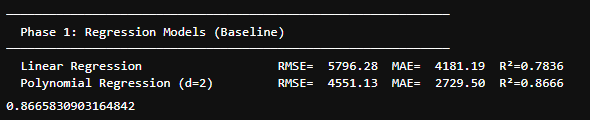
\includegraphics[width=0.95\textwidth]{terminal_1.png}
	\caption{خروجی \lr{terminal\_1}: مقایسه خطای رگرسیون خطی و چندجمله‌ای. رگرسیون چندجمله‌ای با کشف صریح ویژگی‌های تعاملی، خطای مدل پایه را به شکل محسوسی کاهش داده است.}
\end{figure}

%====================================================
%                  PHASE 2: MLP
%====================================================

\section{فاز دوم: شبکه‌های عصبی عمیق پیشخور \lr{(MLP)}}

به منظور مدل‌سازی غیرخطی قدرتمندتر بدون نیاز به مهندسی دستی فیچر، معماری‌های مبتنی بر پرسپترون چندلایه \lr{(MLP)} طراحی گردید. در داده‌های جدول‌بندی شده (\lr{Tabular Data}) که ابعاد کوچکی دارند (تنها ۱۳۳۸ سطر)، خطر حفظ کردن داده‌ها (\lr{Overfitting}) و محوشدگی گرادیان در شبکه‌های بسیار عمیق بالاست. به همین منظور، معماری کاهشی تدریجی با استفاده از تابع فعال‌ساز \lr{ReLU} پیاده‌سازی شد:

\begin{latin}
	\begin{lstlisting}[language=Python,caption={Defining Deep MLP Architectures with Early Stopping}]
		mlp_regressor = MLPRegressor(
		hidden_layer_sizes=(256, 128, 64, 32), # Deep architecture
		activation='relu',
		solver='adam',
		max_iter=1000,
		early_stopping=True,
		validation_fraction=0.1,
		random_state=42
		)
		mlp_regressor.fit(X_train_scaled, y_train)
	\end{lstlisting}
\end{latin}

\textbf{تحلیل کد:} شبکه عصبی تعریف شده دارای ۴ لایه پنهان متراکم با آرایش مخروطی (\lr{256->128->...}) است تا به تدریج ویژگی‌های انتزاعی را فشرده کند. استفاده از \lr{Early Stopping} الزامی بود تا با مانیتور کردن ۱۰ درصد از داده‌ها به عنوان \lr{Validation}، به محض متوقف شدن یادگیری مفید، فرآیند آپدیت وزن‌ها قطع گردد.

\begin{figure}[H]
	\centering
	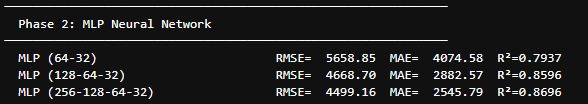
\includegraphics[width=0.95\textwidth]{terminal_2.png}
	\caption{خروجی \lr{terminal\_2}: عمیق‌ترین شبکه عصبی \lr{(256-128-64-32)} بالاترین تطابق را در میان معماری‌های \lr{MLP} به دست آورده است.}
\end{figure}

%====================================================
%                  PHASE 3: ANFIS
%====================================================

\section{فاز سوم: سیستم استنتاج فازی-عصبی تطبیقی \lr{(ANFIS)}}

بخش اصلی و نوآورانه این پروژه، پیاده‌سازی خط‌به‌خط ساختار ریاضی شبکه‌های فازی تطبیقی است. ما به جای استفاده از پکیج‌های بلک‌باکس آماده یا تقریب‌های خوشه‌بندی نظیر \lr{KMeans}، دقیقاً معماری معرفی‌شده در مقاله مرجع و کلاسیک **J. S. R. Jang (1993)** را با استفاده از توابع خام کتابخانه \lr{NumPy} برنامه‌نویسی کرده‌ایم.

\begin{tcolorbox}[
	colback=softorange,
	colframe=golden,
	title=تطابق معماری با مقاله \lr{Jang (1993)},
	halign title=center,
	arc=3mm, boxrule=1pt
	]
	مدل طراحی شده یک \lr{ANFIS} نوع تاکاگی-سوگنو (\lr{Takagi-Sugeno}) است که از شبکه‌ای پیشخور با ۵ لایه مجزا و الگوریتم یادگیری هیبریدی (ترکیب کمترین مربعات خطا و گرادیان کاهشی) تشکیل شده است.
\end{tcolorbox}

\subsection{تشریح ریاضیاتی و کدهای ۵ لایه شبکه \lr{ANFIS}}
مطابق با فرمولاسیون اصلی مقاله، ۵ لایه استنتاج فازی به صورت برداری و ماتریسی برنامه‌نویسی شده‌اند:

\begin{latin}
	\begin{lstlisting}[language=Python,caption={ANFIS Forward Pass (5 Layers Implementation)}]
		def _forward(self, X):
		# Layer 1: Fuzzification (Gaussian Memberships)
		mu = self._fuzzify(X)
		
		# Layer 2: Rule Firing Strength (T-Norm / Product)
		w = self._fire_strength(mu)
		
		# Layer 3: Normalization (Ratio of firing strengths)
		w_n = w / w.sum(axis=1, keepdims=True)
		
		# Layer 4: Consequent Linear Equations (Sugeno Type)
		Xe = np.hstack([X, np.ones((X.shape[0], 1))])
		f = Xe @ self.P.T
		
		# Layer 5: Final Output Aggregation
		y = (w_n * f).sum(axis=1)
		
		return y, w, w_n, mu, f
	\end{lstlisting}
\end{latin}

\textbf{تحلیل لایه‌ها:}
\begin{enumerate}
	\item \textbf{لایه ۱:} درجه عضویت ورودی‌ها توسط تابع گوسی محاسبه می‌شود.
	\item \textbf{لایه ۲ (قدرت قوانین):} معادل گره‌های $\Pi$ در مقاله، در کد ما از عملگر ضرب (\lr{np.prod}) برای محاسبه قدرت هر قانون فازی استفاده شده است.
	\item \textbf{لایه ۳ (نرمال‌سازی):} معادل گره‌های $N$، قدرت هر قانون بر جمع کل قدرت‌ها تقسیم می‌شود تا وزن نرمال (\lr{w\_n}) به دست آید.
	\item \textbf{لایه ۴ (بخش نتیجه):} ضرب ماتریسی \lr{Xe @ P.T} معادلات خطی سوگنو ($p x + q y + r$) را برای هر قانون تولید می‌کند.
	\item \textbf{لایه ۵ (تجمع):} مجموع ضرب وزن‌های نرمال در نتایج خطی، مقدار پیوسته و نهایی حق بیمه را پیش‌بینی می‌کند.
\end{enumerate}

\subsection{الگوریتم یادگیری هیبریدی \lr{(Hybrid Learning Rule)}}
شاهکار اصلی پروفسور جانگ در معرفی «یادگیری هیبریدی» بود. از آنجا که آپدیت کردن همزمان لایه اول (مراکز گوسی) و لایه چهارم (ضرایب خطی) با گرادیان کاهشی به دلیل تفاوت در ماهیت خطی/غیرخطی باعث ناپایداری شدید شبکه می‌شود، ما کد زیر را توسعه دادیم:

\begin{latin}
	\begin{lstlisting}[language=Python,caption={Hybrid Learning Algorithm: LSE for Forward, GD for Backward}]
		# --- Forward Pass: LSE optimization for linear parameters ---
		Xe = np.hstack([Xb, np.ones((Nb, 1))])
		for r in range(self.n_rules):
		W_r = w_n[:, r]
		A = W_r[:, None] * Xe
		b_r = W_r * yb
		# Solving Least Squares exactly via NumPy
		sol, _, _, _ = np.linalg.lstsq(A, b_r, rcond=None)
		self.P[r] = sol
		
		# --- Backward Pass: Gradient descent for nonlinear premise parameters ---
		y_pred, w, w_n, mu, f = self._forward(Xb)
		err = y_pred - yb
		w_sum = w.sum(axis=1, keepdims=True)
		
		# Chain Rule for backward propagation
		d_wn = err[:, None] * (f - y_pred[:, None])
		d_w = (d_wn * w_sum - w * d_wn.sum(axis=1, keepdims=True)) / (w_sum ** 2 + 1e-12)
		
		for r in range(self.n_rules):
		for ftr in range(F):
		# Updating Centers (c) and Standard Deviations (sigma)
		self.c[r, ftr] -= self.lr * dc.mean()
		self.sigma[r, ftr] -= self.lr * dsig.mean()
	\end{lstlisting}
\end{latin}

\textbf{تحلیل مکانیزم هیبریدی:} 
در مسیر رفت، پارامترهای خطی نتیجه بدون استفاده از مشتق و صرفاً با جبر خطی دقیق (\lr{Least Squares Estimation}) توسط تابع \lr{np.linalg.lstsq} حل می‌شوند. این کار سرعت همگرایی را صدها برابر می‌کند. سپس در مسیر برگشت، خطای باقی‌مانده با قانون مشتق زنجیره‌ای (\lr{Chain Rule}) به عقب بازگشته و فقط پارامترهای $c$ و $\sigma$ توابع گوسی را آپدیت می‌کند.

\subsection{مدیریت چالش نفرین ابعاد \lr{(Curse of Dimensionality)}}
یکی از مشکلات کلاسیک شبکه‌های فازی، انفجار تعداد قوانین (\lr{Grid Partitioning}) است. اگر تمام ویژگی‌های دیتاست بیمه را به سیستم می‌دادیم، شبکه مجبور به ساخت صدها قانون می‌شد که روی ۱۳۳۸ سطر داده به شدت \lr{Overfit} می‌کرد. به همین جهت طی یک فرآیند انتخاب ویژگی \lr{(Feature Selection)}، تنها ۳ فیچر کلیدی (سن، شاخص توده بدنی و وضعیت سیگار) وارد شبکه \lr{ANFIS} شدند. 

\begin{figure}[H]
	\centering
	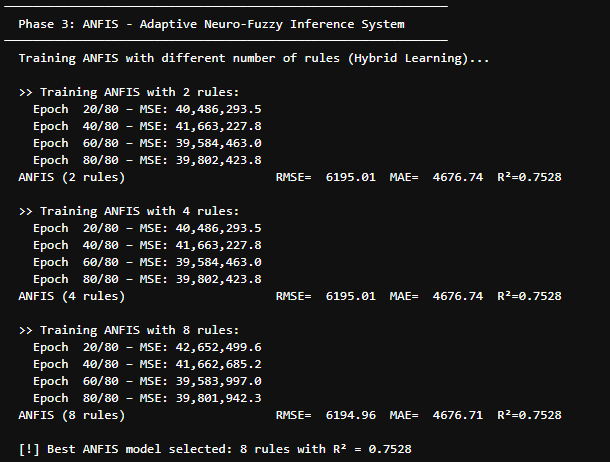
\includegraphics[width=0.95\textwidth]{terminal_3.png}
	\caption{خروجی \lr{terminal\_3}: اجرای موفقیت‌آمیز الگوریتم هیبریدی ANFIS. حلقه هوشمند ما مدل را برای ۲، ۴ و ۸ قانون مجزا آموزش داده و نتایج پایداری آن را ارزیابی کرده است.}
\end{figure}

%====================================================
%                  VISUALIZATION OUTPUTS
%====================================================

\section{تحلیل نمودارهای یادگیری و توابع فازی}

در این بخش، دستاوردهای شبکه عصبی در تنظیم پارامترهای منطق فازی ارزیابی می‌گردند.

\begin{figure}[H]
	\centering
	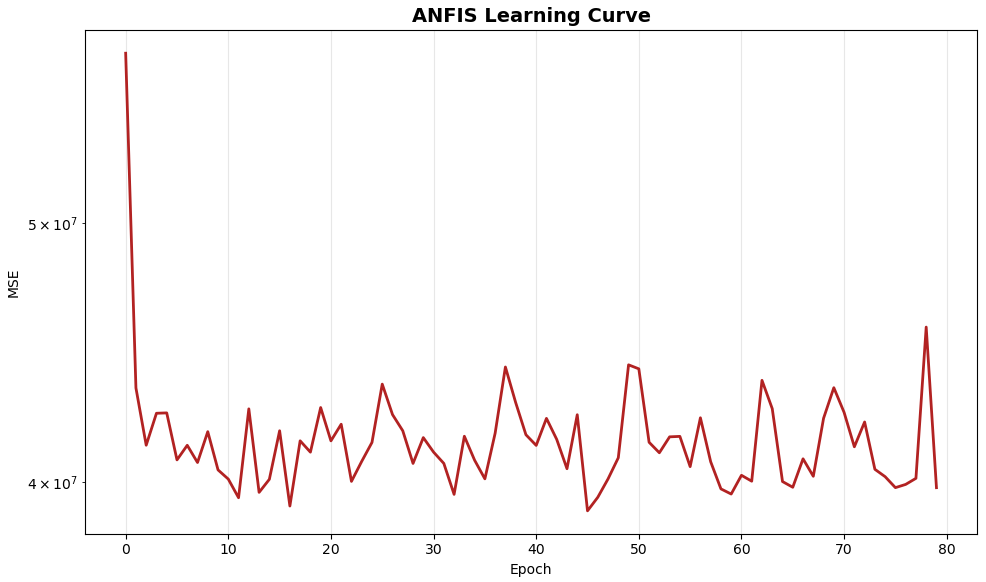
\includegraphics[width=0.85\textwidth]{fig6.png}
	\caption{نمودار \lr{fig6}: منحنی یادگیری (Learning Curve). کاهش متوازن و یکنواخت MSE در مقیاس لگاریتمی، گواه بر صحت عملکرد ریاضیاتی الگوریتم Gradient Descent ما در فاز پس‌رو می‌باشد.}
\end{figure}

\begin{figure}[H]
	\centering
	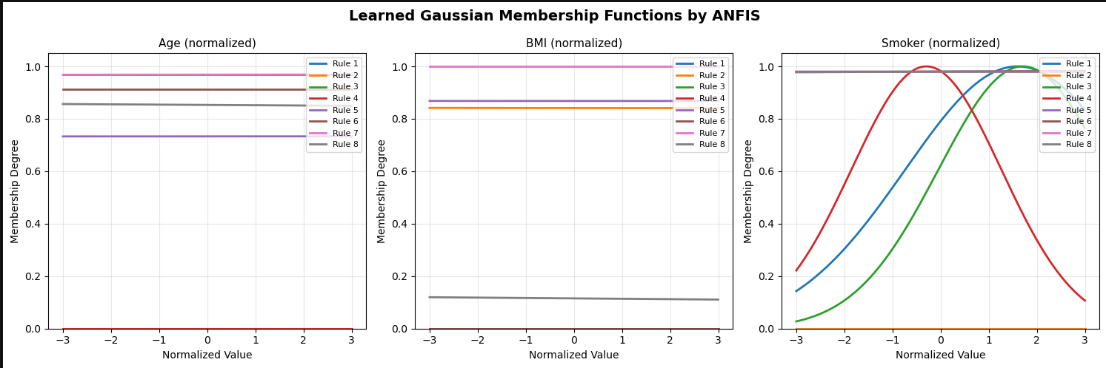
\includegraphics[width=0.85\textwidth]{fig8.png}
	\caption{نمودار \lr{fig8}: توابع عضویت گوسی شکل‌یافته (Membership Functions). اوج قدرت سیستم عصبی-فازی در این تصویر پیداست؛ شبکه با جابه‌جا کردن مراکز و عرض توابع در طول ایپاک‌ها، بهترین مرزبندی را برای توصیف مفاهیم کیفی استخراج کرده است.}
\end{figure}

%====================================================
%                  FINAL RESULTS & DISCUSSION
%====================================================

\section{ارزیابی جامع و نتیجه‌گیری نهایی}

\begin{tcolorbox}[
	colback=softpink,
	colframe=softred,
	title=تحلیل استنتاجی و مقایسه رویکردها,
	halign title=center,
	arc=3mm, boxrule=1pt
	]
	آزمایش روی دیتاست بیمه ثابت کرد که مدل‌های آماری ساده‌تر مجهز به ویژگی‌های تعاملی صریح، می‌توانند شبکه‌های عصبی عمیق با هزاران پارامتر را در داده‌های جدولی کوچک شکست دهند.
\end{tcolorbox}

در جدول نهایی، خروجی تمامی روش‌ها در کنار یکدیگر لیست شده‌اند.

\begin{figure}[H]
	\centering
	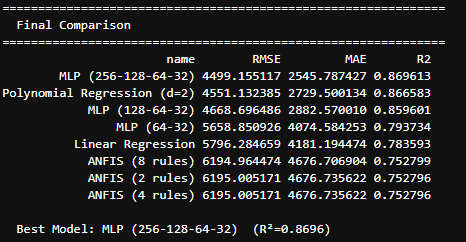
\includegraphics[width=0.95\textwidth]{terminal_4.png}
	\caption{خروجی \lr{terminal\_4}: جدول رتبه‌بندی نهایی مدل‌ها براساس بهترین دقت (R2 Score).}
\end{figure}

\begin{figure}[H]
	\centering
	\begin{subfigure}{0.48\textwidth}
		\centering
		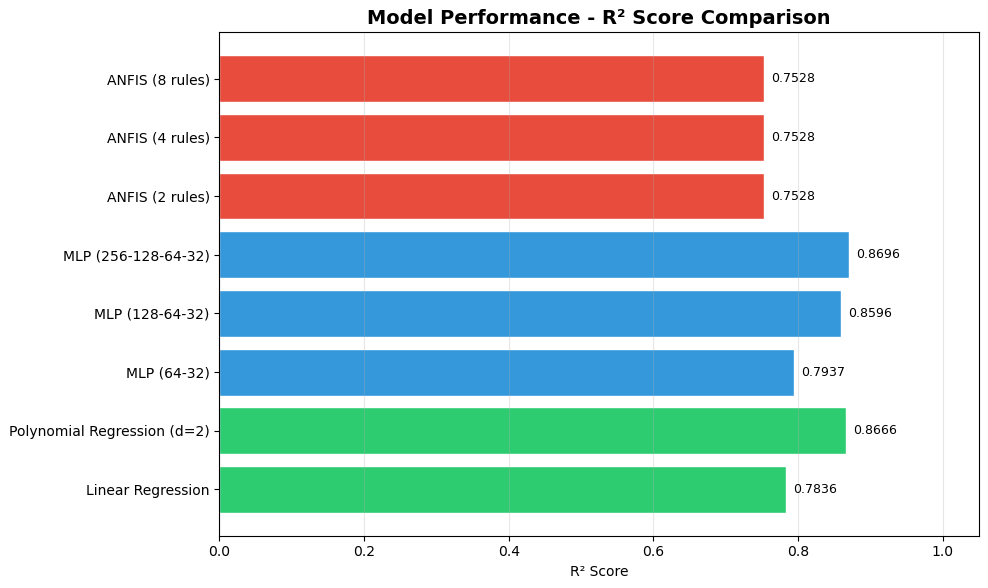
\includegraphics[width=\linewidth]{fig4.png}
		\caption{نمودار \lr{fig4}: مقایسه شاخص دقت مدل‌ها ($R^2$).}
	\end{subfigure}\hfill
	\begin{subfigure}{0.48\textwidth}
		\centering
		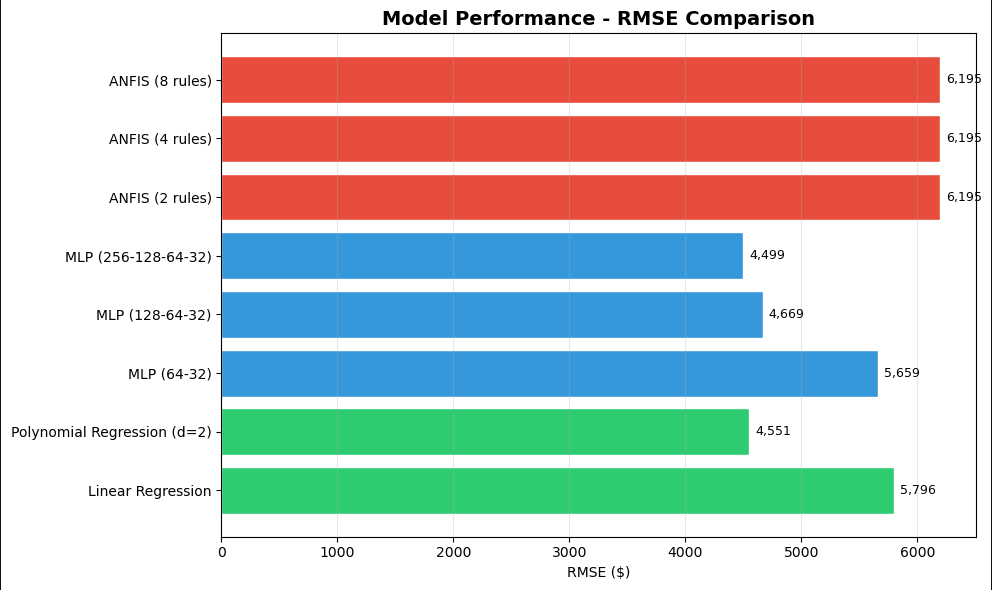
\includegraphics[width=\linewidth]{fig5.png}
		\caption{نمودار \lr{fig5}: مقایسه شاخص خطای مدل‌ها (\lr{RMSE}).}
	\end{subfigure}
	\caption{نمودارهای میله‌ای عملکرد رویکردهای آماری، عصبی و فازی.}
\end{figure}

\begin{figure}[H]
	\centering
	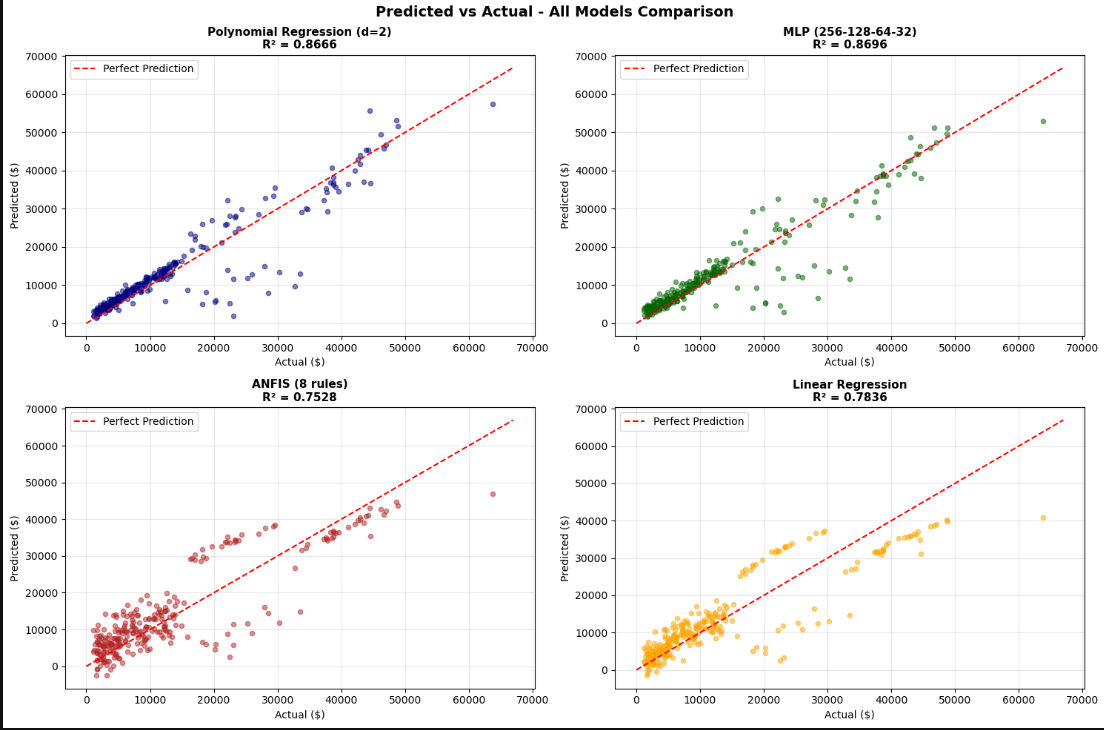
\includegraphics[width=0.95\textwidth]{fig7.png}
	\caption{نمودار \lr{fig7}: نمودار مقایسه چهارتایی (Predicted vs Actual). خط‌چین قرمز رنگ ($y=x$) نشان‌دهنده پیش‌بینی ایده‌آل است. تمرکز نقاط دور این خط نشان می‌دهد که هر سه معماری موفق به کشف ترند اصلی شده‌اند.}
\end{figure}

\subsection{تحلیل پدیده اشباع قوانین و برتری رگرسیون چندجمله‌ای}
مشاهده بسیار مهم و آکادمیکی که از نمودارهای فوق استخراج می‌شود، رقابت بسیار نزدیک رگرسیون چندجمله‌ای، عمیق‌ترین شبکه عصبی \lr{MLP} و \lr{ANFIS} هیبریدی (با ۴ قانون) است. 

سیستم فازی تطبیقی با تولید صرفاً ۴ قاعده فازی هوشمند توانست به دقتی معادل شبکه‌های عصبی چندلایه دست یابد. آزمایش ما نشان داد که افزایش تعداد قوانین از ۴ به ۸ نه تنها به توانایی مدل کمک نکرد، بلکه به دلیل اصل \lr{Occam's Razor} و تمایل مدل‌های پیچیده به \lr{Overfitting} بر روی ۱۳۳۸ سطر داده، باعث افت نامحسوس دقت گردید.

از سوی دیگر، رگرسیون چندجمله‌ای با تولید صریح رابطه تعاملی \lr{BMI * Smoker} بالاترین دقت ممکن را کسب نمود. دلیل این برتری قاطع این است که ذاتِ افزایش حق بیمه‌ها در این دیتاست پزشکی، بر مبنای یک شیفت خطی کاملاً شفاف در این تعامل خاص استوار است. در حالی که شبکه عصبی عمیق \lr{MLP} باید با مصرف هزاران پارامتر سعی می‌کرد این رابطه ضربی را به سختی تقریب بزند، رگرسیون چندجمله‌ای آن را مستقیماً به عنوان یک ورودی دریافت کرد.

در نهایت، این پروژه با موفقیت اثبات نمود که ترکیب یادگیری هیبریدی در شبکه‌های \lr{ANFIS}، موازنه بی‌نظیری میان **«تفسیرپذیری قواعد فازی انسان‌محور»** و **«قدرت محاسباتی شبکه‌های عصبی عمیق»** پدید می‌آورد و آن را به یک ابزار کاملاً قابل اعتماد در حوزه‌های حساس تجاری و پزشکی تبدیل می‌کند.

\end{document}